\section{Optimal vaccine allocation}\label{sec:vaccine_allocation}
The exercise to allocate vaccines across countries raises the need to specify the number of available vaccine shots. We see the number of available vaccines at any time $t$ as exogenous and calibrate it based on the true number of COVID-19 vaccines that have been allocated to the EU.
\begin{figure}[h!]
\centering
\includegraphics[scale=0.3]{images/overview_vaccine_inflow.png}\\
\begin{flushleft}
\scriptsize{\textit{Note}: Solid lines indicate vaccine allocations to a country. Shots below a box indicate the type of vaccines. The formulas next to the solid lines indicate the respective fractions of vaccines that are assigned to the country. The fractions depend on a parameter vector $\theta_l$, over which we optimize to find the optimal solution.}
\end{flushleft}
\caption{Vaccine inflow and allocation across countries}
\label{fig:model_vaccine_allocation}
\end{figure}

Let $W_{l,j}(t)$ be the number of vaccination shots of vaccine $l$ available at time $t$ in country $j$ and $W_l(t) = W_{l,A}(t) + W_{l,B}(t)$ be the the total number of available vaccine $l$ shots at $t$. We assume that all vaccine shots are vaccinated immediately.
\begin{assumption}
\label{ass:vacc_immediately}
The total number of vaccine $l$ available in country $j$ equals the number of vaccinated individuals for all $t \in [0, T]$. 
\begin{align}
\label{eq:vaccine_country}
W_{l,j}(t) &= \phi_{l, j} \cdot \num(\neg X_D, C_j, U_0)  . 
\end{align}
\end{assumption}
\noindent In the real-world, vaccinations take around 2 weeks to yield full protection \citep{cdc.2021}. With this regard, our model can be interpreted such that the number of lately vaccinated individuals is actually the number of individuals that lately received full protection by the vaccine. The vaccination constant would then be the constant defining the reaction of becoming protected. \\

At each point in time $t$, country A receives a fraction $f_{l}(\theta_l; t)$, with $f_{l}: \R^{z} \times [0, \tau] \to [0,1]$, of vaccine $W_l$. The fraction depends on the time $t$ and a parameter vector $\theta_l \in \R^{z}$ that parameterizes $f_{l}(\theta_l; t)$.\\

We assume that all vaccines stay within the two countries and no vaccines are wasted
\begin{assumption}
\label{ass:no_waste}
The total number of vaccine shots of country $j$ is equal to the number shots assigned to it
\begin{align}
\label{eq:vaccine_frac}
W_{l,A}(t) &= f_{l}(\theta_l; t) W_l(t) \\
W_{l,B}(t) &= \left[1 - f_{l}(\theta_l; t)\right] W_l(t) \notag.
\end{align}
\end{assumption}
\noindent We use Assumption \ref{ass:vacc_immediately}, Assumption \ref{ass:no_waste}, and solve for the vaccination constants. They depend on the vaccine inflow, the fraction of vaccine assigned to the respective country, and the total numbers of individuals that potentially can be vaccinated within the country
\begin{align*}
\phi_{l,A} &= \frac{ f_{l}(\theta_l; t) W_{l}(t)}{\num(\neg X_D, C_A, U_0) } \notag \\
\phi_{l,B} &= \frac{\left[1 - f_{l}(\theta_l; t)\right]  W_{l}(t)}{\num(\neg X_D, C_B, U_0)}.
\end{align*}
Note that the vaccination constant is actually not a constant since it depends on time dependent parameters. This is, however, just a naming convention has no further implications for our model.

\subsection{Objective function}
Given a functional form of $f_{l}$, a specific $\bar{\theta}_l \in  \R^z$ is called a \textit{strategy} for vaccine $l$. A \textit{vaccination strategy} $\bar \Theta = \begin{pmatrix}
\bar \theta_1 \\ \bar \theta_2
\end{pmatrix}$ is a collection of strategies defined for both vaccines $l$. We label the strategy $\Theta_{EU}$ that assigns the relative population size of country A to be the fraction of vaccines assigned to country A,
\begin{align}
f_l(\theta_{EU}, t) = \frac{y_0(\neg X_D, C_A)}{y_0(\neg X_D)},
\end{align}
as \textit{current EU strategy} or \textit{current strategy} \citep{ec.2021}. Within the real-world, member states of the EU can refrain from buying their whole quantity and therefore other member states can decide to buy it. We account for this implicitly within our optimization. Since every allocation can be seen as a case where one country waives its right for a certain amount of shots. However, further research could concern incorporating a more game theoretical approach of competing countries.\\

We denote the number of deceased individuals in country A, conditioned on the current strategy, by $y_T(X_D, C_A; \Theta_{EU})$ and the corresponding number in country B by $y_T(X_D, C_B; \Theta_{EU})$.  We use this strategy as baseline case to examine how we can improve using an optimal strategy. An optimal strategy $\Theta^*$ is the solution to the minimization problem
    \begin{argmini!}|l|
	  {\Theta \in \R^{2z}}{y_T(X_D) \notag}{}{}
	  \addConstraint{\phi_{l,A}}{=\frac{ f_{l}(\theta_l; t) W_{l}(t) \tag{C.1}}{\num(\neg X_D, C_A, U_0) } \quad}{\textrm{for } l \in \{1,2\}}
	  \addConstraint{\phi_{l,B}}{= \frac{\left[1 - f_{l}(\theta_l; t)\right]  W_{l}(t)}{\num(\neg X_D, C_B, U_0)} \tag{C.2}\quad}{\textrm{for } l \in \{1,2\}}
	  \addConstraint{\Theta} {= \begin{pmatrix}
\theta_1' & \theta_2'
\end{pmatrix}' \tag{C.3}}{}
	  \addConstraint{}{\beta, \eta, \gamma, \delta_{k,l}, \omega_{k,l}, Y(0), W_{l}(t) \tag{C.4}}{}
     \end{argmini!}
and we call it \textit{optimal vaccination strategy} with respect to the given minimization problem. Conditions $C.1$, $C.2$, and $C.3$ indicate how the parameter vector $\Theta$ affects the model. $C.4$ specifies that all exogenous parameters are set to a constant value or exogenous function.

If additionally constraints $C.5$ and $C.6$ are satisfied, 
\begin{align}
y_T(X_D, C_A) &< y_T(X_D, C_A; \Theta_{EU}) \tag{C.5} \\
y_T(X_D, C_B) &< y_T(X_D, C_B; \Theta_{EU}) \tag{C.6}
\end{align}
the optimal strategy is Pareto optimal and we call it \textit{Pareto optimal vaccination strategy}. The Pareto optimality conditions ensure that both countries have less deceased individuals as within the current strategy. Taking the perspective that both countries can veto against strategies, non Pareto optimal strategies might not be implementable since no country would agree to deviate from the current strategy if it experiences more deceased individuals with the new strategy.\\

As objective we choose the total number of deceased individuals. Other objectives like the total number of infectious individuals, or some combination of both, could be considered as well. We decided to choose the total number of deaths such that the death protection parameters $\omega_{k,l}$ influence the solution. \\

\subsection{Functional form of the vaccine allocation}
We examine two functional forms of $f_{l}$. First, $f_{l}$ is a stepwise function. Second, $f_{l}$ is a logistically transformed third order spline function. Both forms can be parameterized using the parameter vector $\theta_l$. Both forms do not yield constructive vaccination strategies since we do not link the vaccine allocation directly to the state of the model but rather optimize over time dependent parameter.\\

To define the functional forms, we subdivide the interval $[0,T]$ into a tagged partition $0=t_0 < t_1 < \dots < t_z = T$. Let $\mathcal{T}_i = [t_{i-1}, t_{i})$, for $i = 1, \dots, z$, be the corresponding intervals of the tagged partition. We label $\mathcal{T}$ as the $i$-\textit{th decision period}. To be more precise on the functional form of $f_l$, we subdivide the parameter vector into its components $\theta_l = \begin{pmatrix}
\theta_{l,1}  & \theta_{l,2} & \dots & \theta_{l,z} \end{pmatrix}'$. \\

\textbf{Stepwise.} In this world, policy makers determine a fraction that is allocated to country A for a fixed decision period $\mathcal{T}_i$, evaluate, and then adjust before the next decision period $T_{i+1}$ begins. In Figure \ref{fig:examples} we show an exemplary vaccination strategy for vaccine $l$.

In mathematical terms, every $\theta_{l,i} \in [0,1]$ is assigned to an interval $\mathcal{T}_i$. The parameters $\theta_{l,i}$ are in this case the fractions of vaccines assigned to country A.
\begin{align}
f_l(\theta_l; t) = \theta_{l,i} \quad \forall t \in \mathcal{T}_i.
\end{align}
%\[ f_{l}(\theta; t) = \begin{cases} 
%      \theta_{l,1} & \textrm{if } t \in T_1 \\
%      \theta_{l,i} & \textrm{if } t \in \mathcal{T}_i \\
%      \theta_{l,z} & \textrm{if } t \in T_z 
%   \end{cases}
%\] 
Note that the current EU strategy is a special case of a step function that has $\theta_{l;1}= \theta_{l,2} = \hdots = \theta_{l,z}=y_0(\neg X_D, C_l)/y_0(\neg X_D)$, assuming that the allocations are not adjusted for changes in the population sizes over the course of the pandemic.
\begin{figure}[h!]
\centering
\includegraphics[scale=0.8]{images/example_methods.png}\\
\begin{flushleft}
\scriptsize{\textit{Note}: Examples of a piecewise vaccine allocation in orange and a spline allocation in blue. The first graph depicts the values of the spline and the second graph shows the corresponding transformed function that maps the values into the unit interval. The third graph shows a different approach using a piecewise constant function. Decision intervals have a duration of 2 weeks.}
\end{flushleft}
\caption{Exemplary vaccination strategies for country A.}
\label{fig:examples}
\end{figure}

\textbf{Splines.} In this world, policy makers decide on the start and end values of the vaccine allocations within each interval $\mathcal{T}_i$. Given the boundary values, one polynomial for each interval $\mathcal{T}_i$ is computed, and logistically transformed to meet the unit interval domain of the fractions. By using polynomials, rather than constant functions, we allow for more complex policy decisions within one decision period $\mathcal{T}_i$ since fluctuations within one decision period can be taken into account. However, one should note that this exercise is rather theoretical and aims to show what strategies could be achieved theoretically.

We use splines instead of a global polynomial interpolation since they are practical with respect to construction and global interpolations might suffer from undesired properties, as in Runge's phenomenon \citep{Runge.1901}.\\
 
%\begin{figure}
\subfloat[]
{
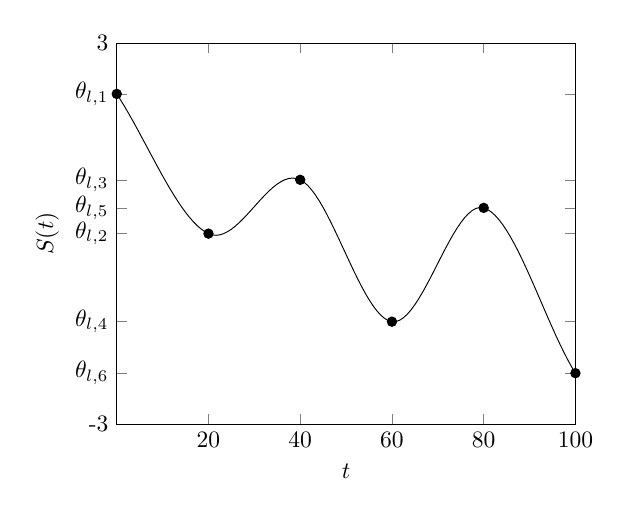
\begin{tikzpicture}[scale=0.85]
     \begin{axis}[xtick={20, 40,...,100}, ytick={-3, -2.1972, -1.3863, 0, 0.4054, 0.8473, 2.2, 3}, yticklabels={-3, $\theta_{l,6}$, $\theta_{l,4}$, $\theta_{l,2}$, $\theta_{l,5}$, $\theta_{l,3}$, $\theta_{l,1}$, 3}, xmin=0, xmax=100,  ymin=-3, ymax=3, xlabel = $t$, ylabel = $S(t)$]

\addplot[domain=0:20] {(2*((x-0)/(20-0))^3 - 3*((x-0)/(20-0))^2 + 1)*(2.2) + (((x-0)/(20-0))^3 - 2*((x-0)/(20-0))^2+((x-0)/(20-0)))*(0-(2.2)) + (-2*((x-0)/(20-0))^3+3*((x-0)/(20-0))^2)*(0) + (((x-0)/(20-0))^3-((x-0)/(20-0))^2)*1/2*((0-2.2) + (0.8473-0)) };
\addplot[domain=20:40] {(2*((x-20)/(40-20))^3 - 3*((x-20)/(40-20))^2 + 1)*0 + (((x-20)/(40-20))^3 - 2*((x-20)/(40-20))^2+((x-20)/(40-20)))*1/2*( (0.8473-0) + (0-(2.2)))+ (-2*((x-20)/(40-20))^3+3*((x-20)/(40-20))^2)*(0.8473) + (((x-20)/(40-20))^3-((x-20)/(40-20))^2)*1/2*((0.8473-0) + (-(1.3863)-0.8473)) };
\addplot[domain=40:60] {(2*((x-40)/(60-40))^3 - 3*((x-40)/(60-40))^2 + 1)*0.8473 + (((x-40)/(60-40))^3 - 2*((x-40)/(60-40))^2+((x-40)/(60-40)))*1/2*( (-(1.3863)-0.8473) + (0.8473-0))+ (-2*((x-40)/(60-40))^3+3*((x-40)/(60-40))^2)*(-(1.3863)) + (((x-40)/(60-40))^3-((x-40)/(60-40))^2)*1/2*((-(1.3863)-0.8473) + (0.4054--(1.3863)))};
\addplot[domain=60:80] {(2*((x-60)/(80-60))^3 - 3*((x-60)/(80-60))^2 + 1)*-(1.3863) + (((x-60)/(80-60))^3 - 2*((x-60)/(80-60))^2+((x-60)/(80-60)))*1/2*( (0.4054--(1.3863)) + (-(1.3863)-0.8473))+ (-2*((x-60)/(80-60))^3+3*((x-60)/(80-60))^2)*(0.4054) + (((x-60)/(80-60))^3-((x-60)/(80-60))^2)*1/2*((0.4054--(1.3863)) + (-2.1972-0.4054))};
\addplot[domain=80:100] {(2*((x-80)/(100-80))^3 - 3*((x-80)/(100-80))^2 + 1)*0.4054 + (((x-80)/(100-80))^3 - 2*((x-80)/(100-80))^2+((x-80)/(100-80)))*1/2*( (-2.1972-0.4054) + (0.4054--(1.3863)))+ (-2*((x-80)/(100-80))^3+3*((x-80)/(100-80))^2)*(-2.1972) + (((x-80)/(100-80))^3-((x-80)/(100-80))^2)*1/2*((-2.1972-0.4054) + (0.2-2.1972))};
\addplot[mark=*] coordinates {(0,2.2)};
\addplot[mark=*] coordinates {(20,0)};
\addplot[mark=*] coordinates {(40,0.8473)};
\addplot[mark=*] coordinates {(60,-1.3863)};
\addplot[mark=*] coordinates {(100,-2.1972)};
\addplot[mark=*] coordinates {(80,0.4054)};
\end{axis}
\end{tikzpicture}
}
\subfloat[ ]
{
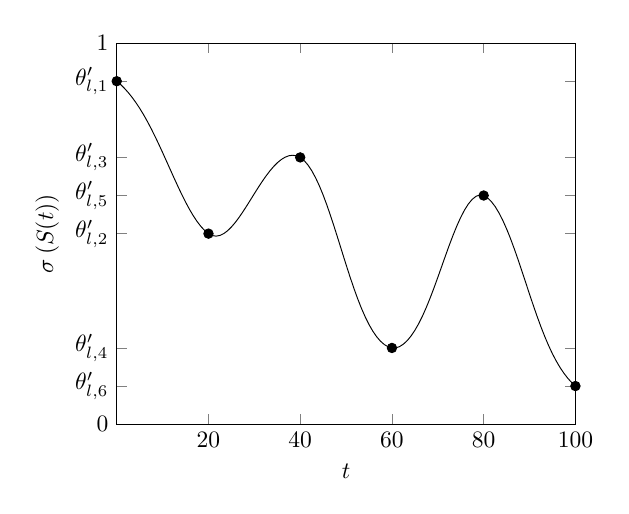
\begin{tikzpicture}[scale=0.85]
    \begin{axis}[xtick={20, 40,...,100}, ytick={0, 0.1, 0.2, 0.5, 0.6, 0.7, 0.9, 1}, yticklabels={0, $\theta_{l,6}'$, $\theta_{l,4}'$, $\theta_{l,2}'$, $\theta_{l,5}'$, $\theta_{l,3}'$, $\theta_{l,1}'$, 1}, xmin=0, xmax=100,  ymin=0, ymax=1, xlabel = $t$, ylabel=$\sigma\left(S(t)\right)$ ]

\addplot[domain=0:20] {1/(1+e^(-((2*((x-0)/(20-0))^3 - 3*((x-0)/(20-0))^2 + 1)*(2.2) + (((x-0)/(20-0))^3 - 2*((x-0)/(20-0))^2+((x-0)/(20-0)))*(0-(2.2)) + (-2*((x-0)/(20-0))^3+3*((x-0)/(20-0))^2)*(0) + (((x-0)/(20-0))^3-((x-0)/(20-0))^2)*1/2*((0-2.2) + (0.8473-0)) )))};
\addplot[domain=20:40] {1/(1+e^(-((2*((x-20)/(40-20))^3 - 3*((x-20)/(40-20))^2 + 1)*0 + (((x-20)/(40-20))^3 - 2*((x-20)/(40-20))^2+((x-20)/(40-20)))*1/2*( (0.8473-0) + (0-(2.2)))+ (-2*((x-20)/(40-20))^3+3*((x-20)/(40-20))^2)*(0.8473) + (((x-20)/(40-20))^3-((x-20)/(40-20))^2)*1/2*((0.8473-0) + (-(1.3863)-0.8473)) )))};
\addplot[domain=40:60] {1/(1+e^(-((2*((x-40)/(60-40))^3 - 3*((x-40)/(60-40))^2 + 1)*0.8473 + (((x-40)/(60-40))^3 - 2*((x-40)/(60-40))^2+((x-40)/(60-40)))*1/2*( (-(1.3863)-0.8473) + (0.8473-0))+ (-2*((x-40)/(60-40))^3+3*((x-40)/(60-40))^2)*(-(1.3863)) + (((x-40)/(60-40))^3-((x-40)/(60-40))^2)*1/2*((-(1.3863)-0.8473) + (0.4054--(1.3863))) )))};
\addplot[domain=60:80] {1/(1+e^(-((2*((x-60)/(80-60))^3 - 3*((x-60)/(80-60))^2 + 1)*-(1.3863) + (((x-60)/(80-60))^3 - 2*((x-60)/(80-60))^2+((x-60)/(80-60)))*1/2*( (0.4054--(1.3863)) + (-(1.3863)-0.8473))+ (-2*((x-60)/(80-60))^3+3*((x-60)/(80-60))^2)*(0.4054) + (((x-60)/(80-60))^3-((x-60)/(80-60))^2)*1/2*((0.4054--(1.3863)) + (-2.1972-0.4054)) )))};
\addplot[domain=80:100] {1/(1+e^(-((2*((x-80)/(100-80))^3 - 3*((x-80)/(100-80))^2 + 1)*0.4054 + (((x-80)/(100-80))^3 - 2*((x-80)/(100-80))^2+((x-80)/(100-80)))*1/2*( (-2.1972-0.4054) + (0.4054--(1.3863)))+ (-2*((x-80)/(100-80))^3+3*((x-80)/(100-80))^2)*(-2.1972) + (((x-80)/(100-80))^3-((x-80)/(100-80))^2)*1/2*((-2.1972-0.4054) + (0.2-2.1972)) )))};
\addplot[mark=*] coordinates {(0,0.9)};
\addplot[mark=*] coordinates {(20,0.5)};
\addplot[mark=*] coordinates {(40,0.7)};
\addplot[mark=*] coordinates {(60,0.2)};
\addplot[mark=*] coordinates {(100,0.1)};
\addplot[mark=*] coordinates {(80,0.6)};
\end{axis}
\end{tikzpicture}
}
\caption{Exemplary spline (a) and the logistically transformed spline (b)}
\label{fig:splines}
\end{figure}


Figure \ref{fig:examples} shows an exemplary spline and how it is shrinked via the logistic function $\sigma(x)$ into the unit interval, via the logistic function, $\sigma(x)$ to obtain values between zero and one.  %Within the sensitivity analysis we use the hyperbolic tangent function $\tanh(x)$ to examine if the functional choice of the transformation changes our results.
Given a polynomial from the third order polynomial ring over the real numbers $P_{l,i}(t) \in \R_3(t)$, the fraction is mathematically described by the composition of the polynomial and the logistic function
\begin{align}
f_{l}(\theta; t) =  \frac{1}{1 + \exp{(-P_{l,i}(t))}} \quad \forall t \in \mathcal{T}_i. 
\end{align}

We chose $P_{l,i}(t)$ to be in cubic hermite form. The name cubic arises from the condition that every $P_{l,i}(t)$ is maximal a third-order polynomial. The name hermite indicates that the derivatives at the boundaries $P'_{l,i}(t_{i-1})$ are computed using finite differences. We use central finite differences and forward as well as backward finite differences at the respective boundaries $t_0$ and $t_{z}$
\begin{align}
\label{eq:finite_differences}
P'_{l,1}(t_0) &\approx \frac{P_{l,1}(t_1) - P_{l,1}(t_0)}{t_1 - t_0} \\
P'_{l,i}(t_{i-1}) &\approx \frac{1}{2}\left[\frac{P_{l,i}(t_{i}) - P_{l,i}(t_{i-1})}{t_{i} - t_{i-1}} + \frac{P_{l,i-1}(t_{i-1}) - P_{l,i-1}( t_{i-2})}{t_{i-1} - t_{i-2}} \right] \notag \\
P'_{l,z}(t_{z}) &\approx \frac{P_{l,z}(t_{z}) - P_{l,z}(t_{z-1})}{t_{z} - t_{z-1}} \notag 
\end{align}. 

If we have the two functional values at the boundaries and approximations for their derivatives, we have four conditions to specify the polynomial of order three. Thus, we can parameterize the splines by specifying the polynomial values at the boundaries 
\begin{align}
\label{eq:splines_bound_theta}
P_{l,i}(t_{i-1}) &= \theta_{l, i-1} \\
P_{l,i}(t_{i}) &= \theta_{l,i} \notag
\end{align}

The polynomial $P_{l,i}(t) $ is given as a linear combination of four basis polynomials  $B_1(t), B_2(t), B_3(t), B_4(t) \in \R_3(t)$ with the boundary values of the polynomial and its derivative. Let $t' = (t-t_{i-1})/(t_{i} - t_{i-1})$ for $t \in \mathcal{T}_i$ and
\begin{align}
P_{l,i}(t) &= B_1(t') \overbrace{P_{l,i}(t_{i-1})}^{\theta_{l,i-1}} + B_2(t') (t_{i} - t_{i-1}) P'_{l,i}(t_{i-1})  \\& \quad + B_3(t') \underbrace{P_{l,i}(t_{i})}_{\theta_{l,i}} + B_4(t') (t_{i} - t_{i-1}) P'_{l,i}(t_{i}) \quad \forall t \in \mathcal{T}_i. \notag
\end{align}
The scalars of the linear combination are dependent on the parameter vector $\theta_l$ through \eqref{eq:finite_differences} and \eqref{eq:splines_bound_theta}. The basis polynomials are defined by $B_1(t) = 2t^3 - 3t^2 +1, B_2(t) = t^3 - 2t^2 +t, B_3(t) = -2t^3 + 3t^2$ and $B_4(t) = t^3 - t^2$. Note that the imposed structure of $P_{l,i}(t)$ is well-defined, which can be verified by evaluating the polynomial and its derivative at the boundaries $t_{i-1}$ and $t_i$. We provide the calculations in the appendix \ref{A:well_conditioning}.

We show that the basis polynomials indeed form a basis of $\R_3(t)$. Showing the basis property proves that the four polynomials span $\R_3(t)$ and we therefore do not exclude any polynomials from the space of policies that could be implemented.
\begin{theorem}
$B_1(t), B_2(t), B_3(t), B_4(t) \in \R_3(t)$ form a polynomial basis of $\R_3(t)$.
\end{theorem}
\begin{proof}
The proof is moved to the Appendix \ref{A:polynomial_basis}.
\end{proof} 


 
